% !TeX spellcheck = en_GB
%%%%%%%%%%%%%%%%%%%%%%%%%%%%%%%%%%%%%%%%%%%%%%%%%%%%%%%%%%%%%%%%%%%%%%%%%
%%%%%%%% large scale phenomena vertical ? %%%%%%%%%%%%%%
\section{Observation of large scale weather phenomena in the vertical}\label{sec:res:verticalSWC}
%%%%%%%%% image reflectivity %%%%%%%%%%%%%%
\begin{figure}[h!]
	\centering
	% 23/12
	\begin{subfigure}[t]{\textwidth}
		\centering
		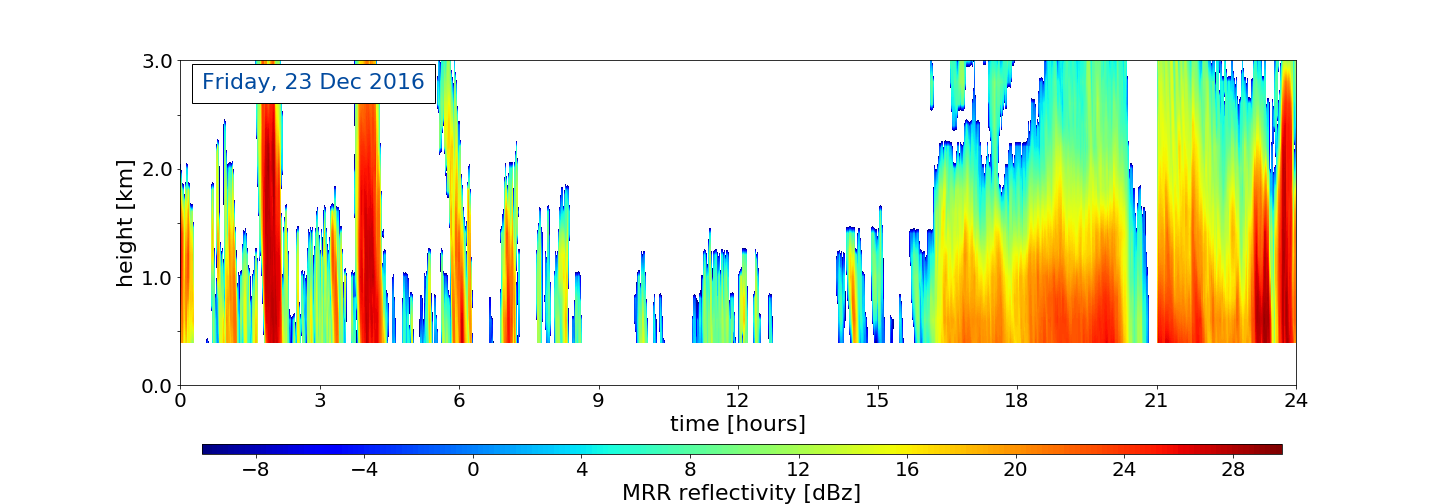
\includegraphics[trim={4.cm 2.5cm 4.5cm 1.5cm},clip,width=0.9\textwidth]{./fig_MRR_refl/MRR_20161223}
		\caption{}\label{fig:ret:refl23}
	\end{subfigure}
	% 25/12
	\begin{subfigure}[t]{\textwidth}
		\centering
		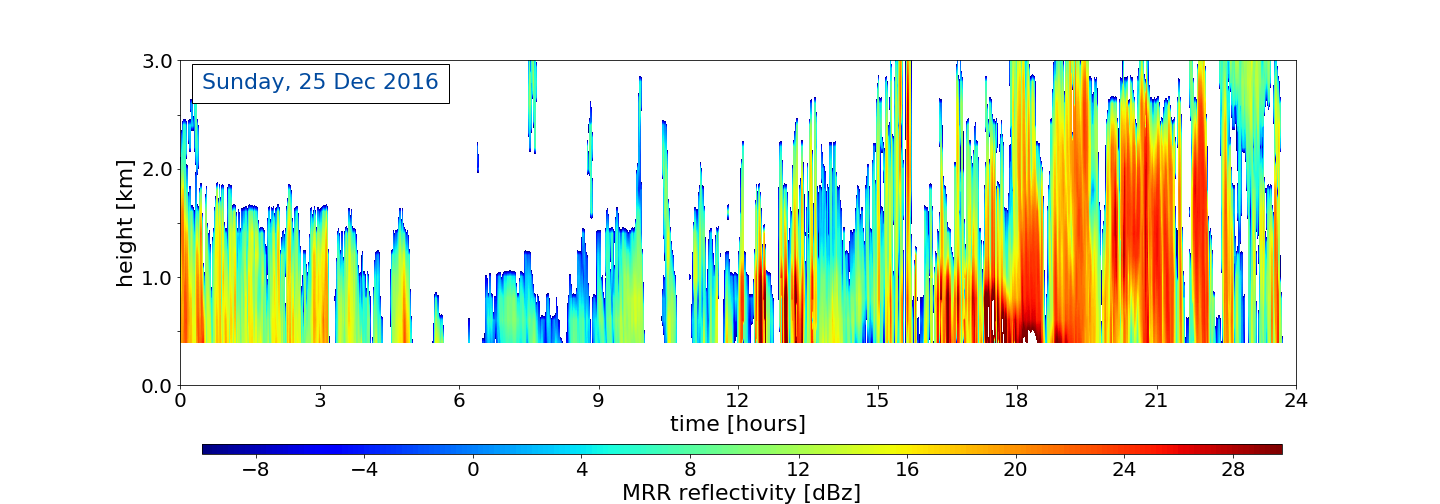
\includegraphics[trim={4.cm 2.5cm 4.5cm 1.5cm},clip,width=0.9\textwidth]{./fig_MRR_refl/MRR_20161225}
		\caption{}\label{fig:ret:refl25}
	\end{subfigure}
	% 26/12
	\begin{subfigure}[t]{\textwidth}
		\centering
		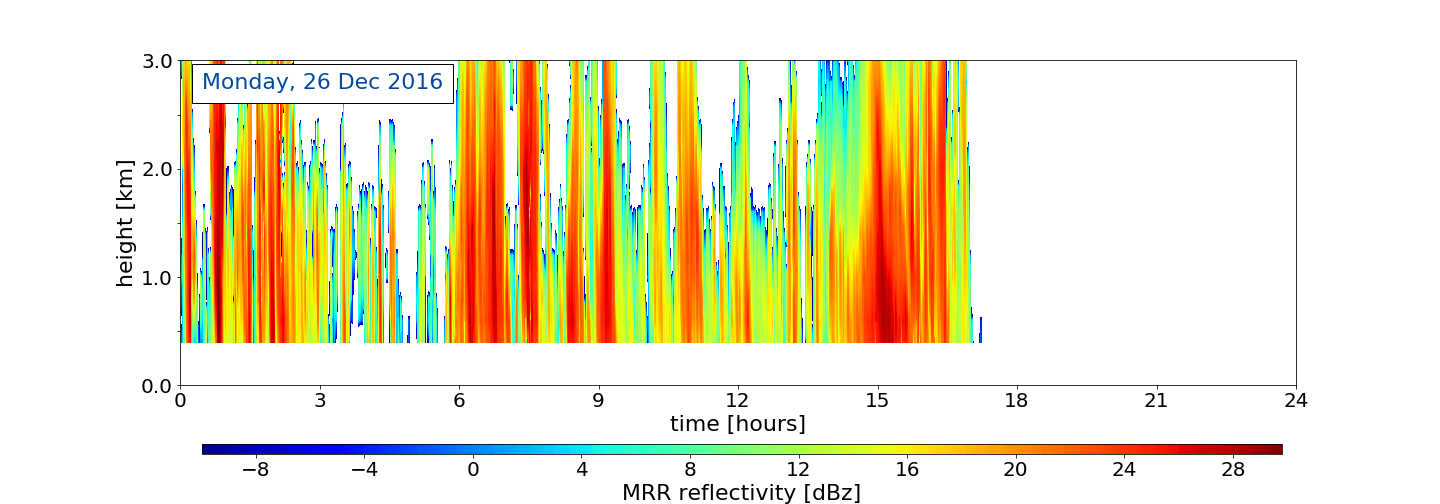
\includegraphics[trim={4.cm 2.5cm 4.5cm 1.5cm},clip,width=0.9\textwidth]{./fig_MRR_refl/MRR_20161226}
		\caption{}\label{fig:ret:refl26}
	\end{subfigure}
	% label
	\begin{subfigure}[t]{\textwidth}
		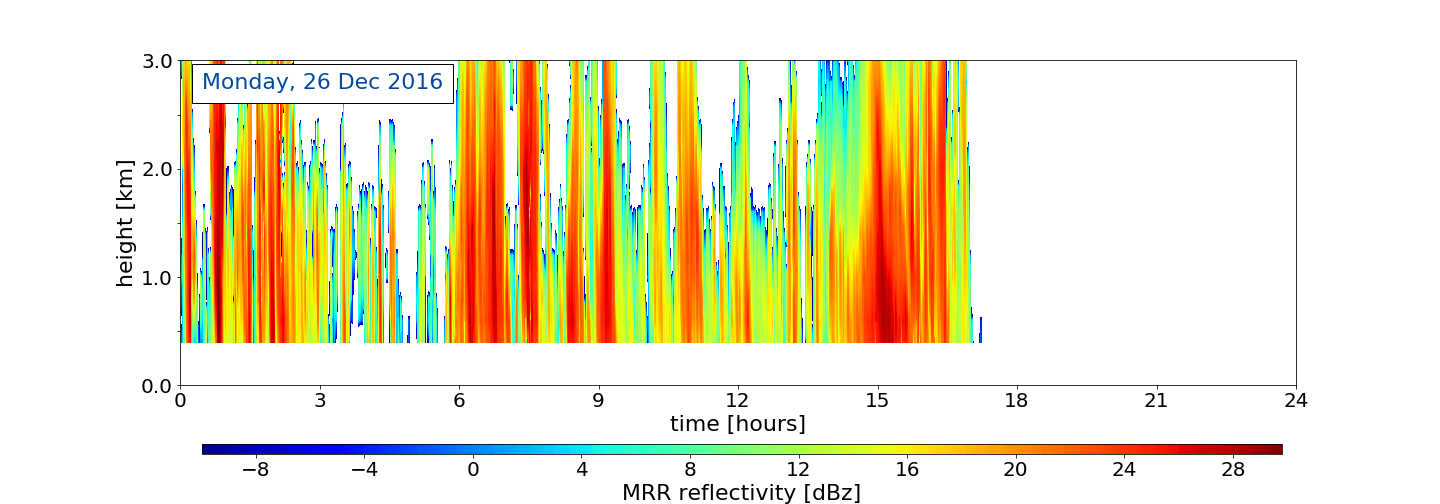
\includegraphics[trim={6.5cm 0cm 5.3cm 15.5cm},clip,width=\textwidth]{./fig_MRR_refl/MRR_20161226}
	\end{subfigure}
	\caption{MRR reflectivity for the days when a front or an occlusion passed through at Haukeliseter. \SI{}{\decibel Z} reflectivity according to the colour bar, with weaker precipitation in blue and more intense precipitation in red. \protect\subref{fig:ret:refl23}: Friday, \SI{23}{\dec}, \protect\subref{fig:ret:refl25}: Sunday, \SI{25}{\dec}, and \protect\subref{fig:ret:refl26}: Monday, \SI{26}{\dec}.}\label{fig:ret:refl}
\end{figure}
%%%%%%%%%%%%%%%%%%%%%%%%%%%%%%%%%%%%%%%%%%%%%%%%%%%%%%%%%%%%%%%%%%%%%%%%%
\noindent
Frontal boundary passages were observed at the surface several times throughout the extreme storm in December 2016. MEPS is able to predict the large scale features for initialisation more than \SI{24}{\hour} before (\Cref{sec:res:large_scale_sfc}). In winter 2016 three additional instruments were installed to estimate the vertical snow water content at Haukeliseter. This unique approach gives the unique opportunity to compare the vertical forecasts of SWC to vertical solid precipitation observations. As far as the author knows is there no study on this particular topic about the verification of vertical ensemble member prediction models with observations.
\\
\Cref{fig:ret:refl} shows the reflectivity from the MRR at Haukeliseter for \SIlist{23;25;26}{\dec}. Passages of occluded fronts and a warm sector were observed on \SIlist{23;26;25}{\dec}, respectively. \Cref{fig:ret:refl26} presents only values until \SI{17}{\UTC}, because of the temperature change and hence a precipitation shift followed liquid drops freezing on the MRR dish and the signal got attenuated. 
%\\
The transit of the boundaries is shown in \Cref{fig:ret:refl} by the more consistent structure of a storm with higher reflectivity values. 
While on \SIlist{23;25}{\dec} the reflectivity did not pass values larger than \SI{28}{\decibel Z} shows \Cref{fig:ret:refl25} high reflectivity values larger than \SI{30}{\decibel Z} (compare for approximation \Cref{tab:ref_values}). These high values indicate the observation of possible liquid precipitation. Images from the MASC were able to verify observed liquid drops (\Cref{fig:res:obs_masc}). 
%\\
%\\
%%%%%%%%% image SWC retrieval MEPS 23 %%%%%%%%%%%%%%
\begin{figure}[t]
	\centering
	% 23/12
	\begin{subfigure}[t]{\textwidth}
		\centering
		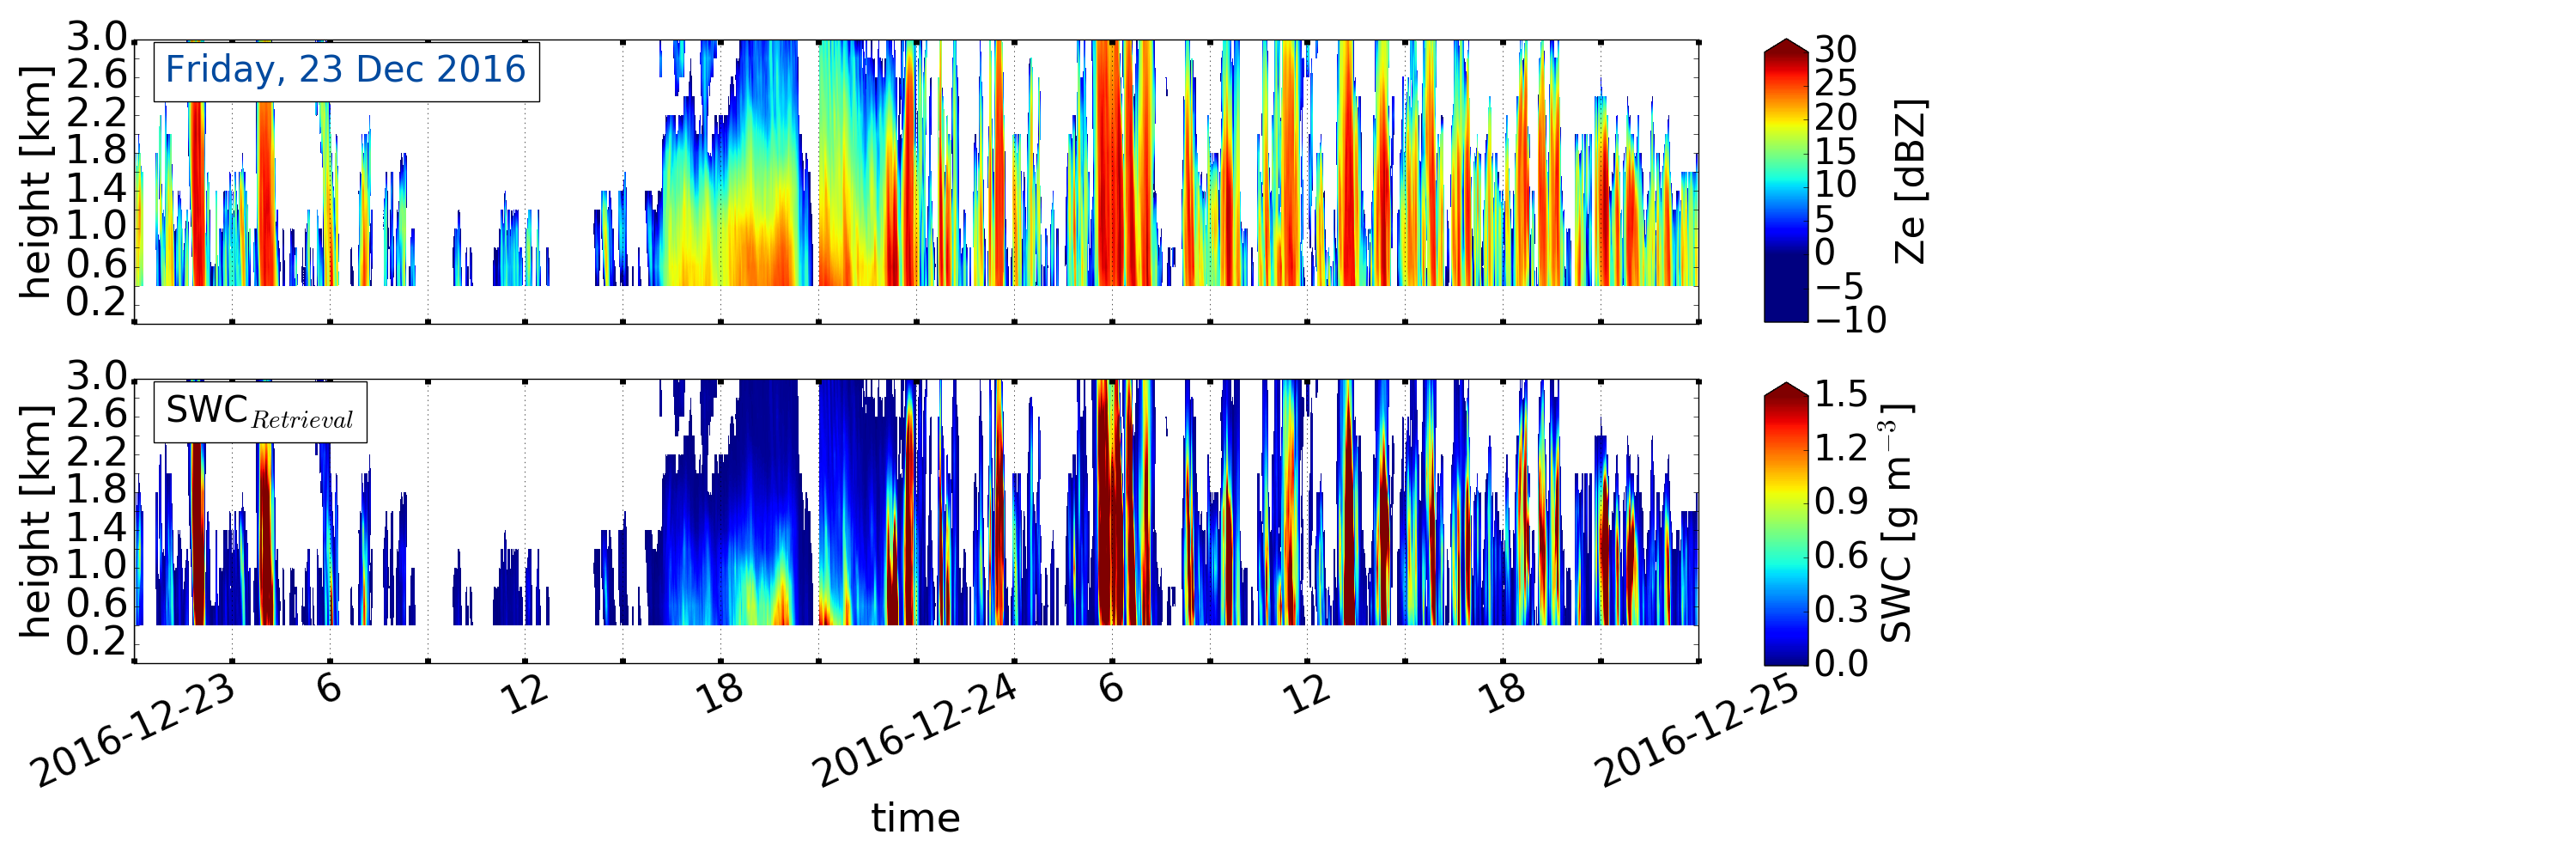
\includegraphics[trim={0.cm 2.2cm 19.cm 0.5cm},clip,width=0.9\textwidth]{./fig_obs_ret/20161223}
		\caption{}\label{fig:SWC:ret_23}
	\end{subfigure}
	% EM
	\begin{subfigure}[t]{\textwidth}
		\centering
		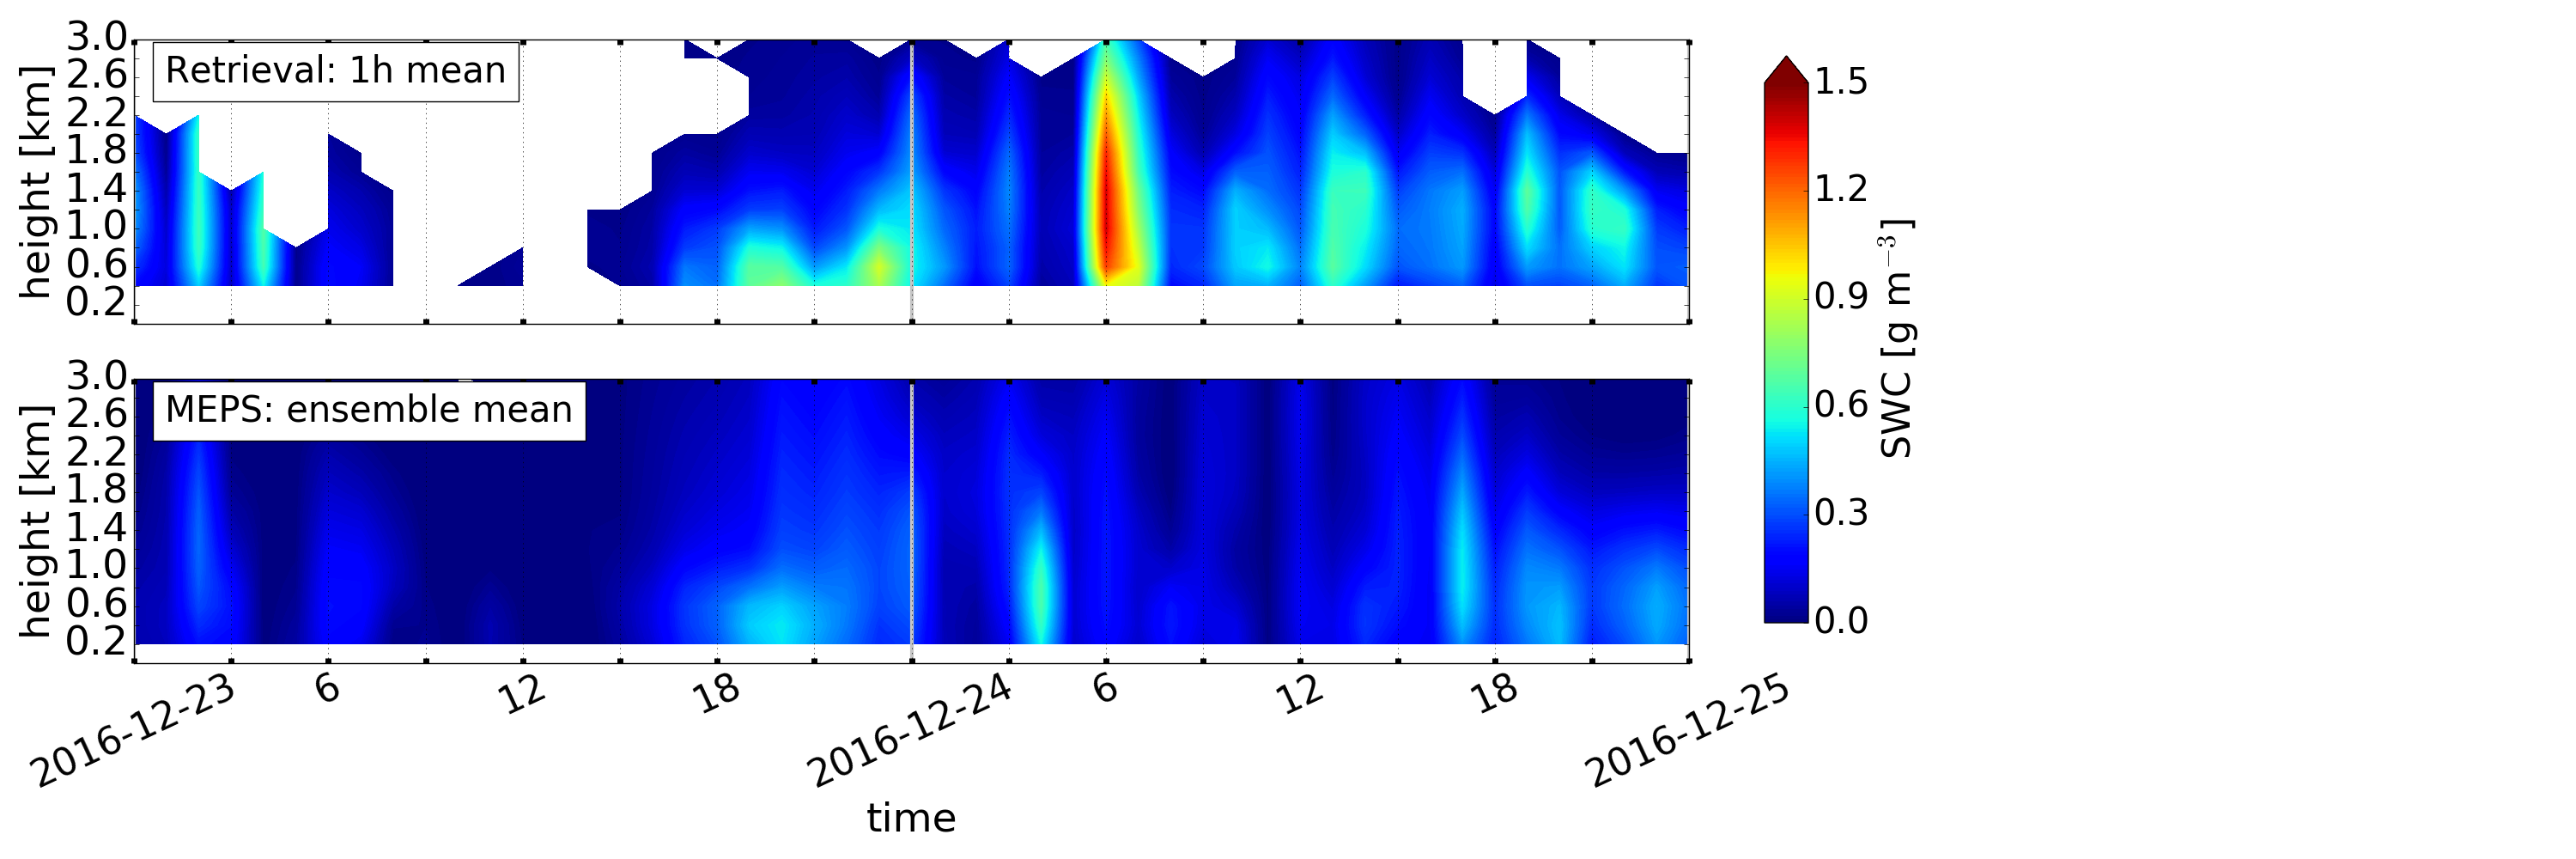
\includegraphics[trim={0.cm 2.2cm 19.cm 0.5cm},clip,width=0.9\textwidth]{./fig_vert_SWC_EM/20161223}
		\caption{}\label{fig:SWC_EM:23}
	\end{subfigure}
	% 3h
	\begin{subfigure}[t]{\textwidth}
		\centering
		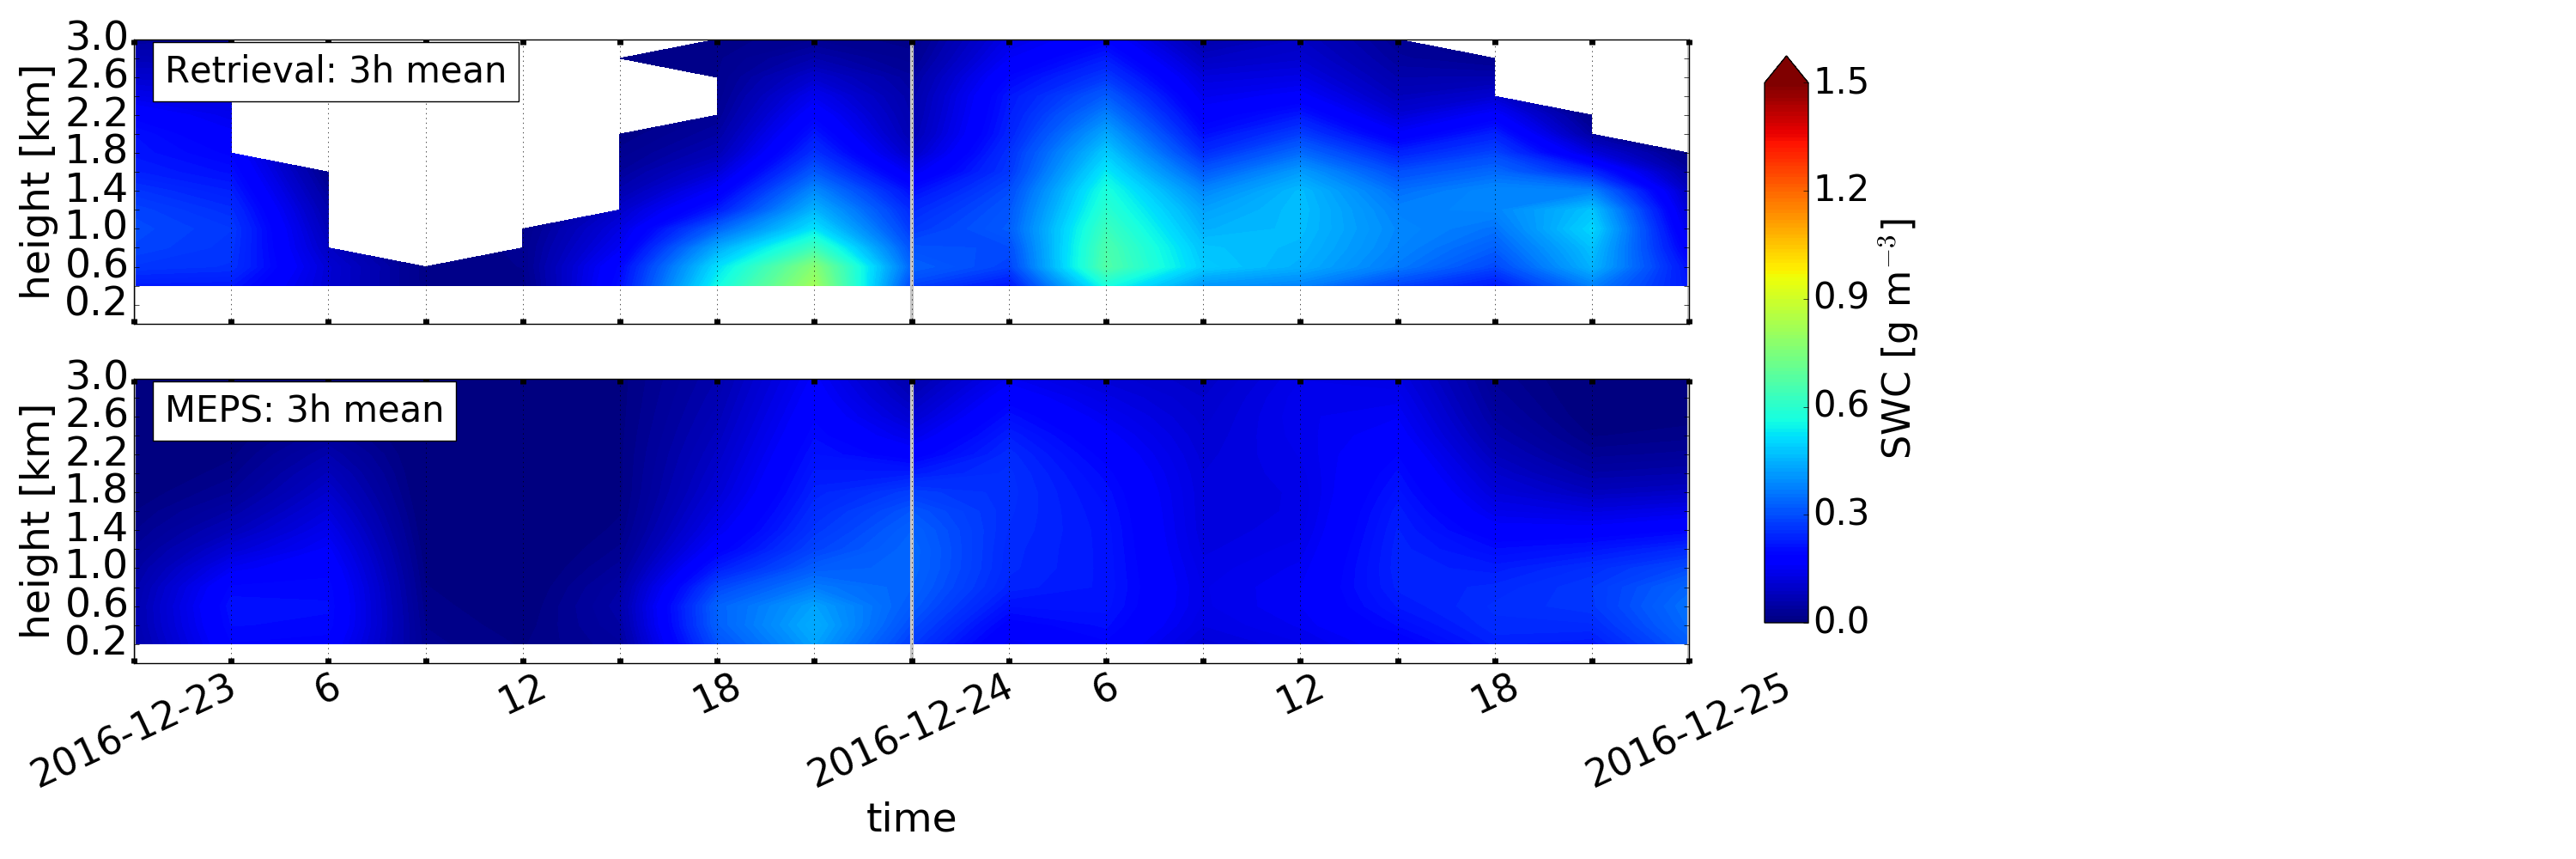
\includegraphics[trim={0.cm 0.8cm 19.cm 0.5cm},clip,width=0.9\textwidth]{./fig_vert_SWC_3h/20161223}
		\caption{}\label{fig:SWC3h:23}
	\end{subfigure}
	\caption{Initialisation \SIlist{23;25;26}{\dec} \SI{0}{\UTC}. 
		(\protect\subref{fig:SWC:ret_23}, \protect\subref{fig:SWC:ret_25}, \protect\subref{fig:SWC:ret_26}) Upper panel: MRR reflectivity for \SI{48}{\hour}, lower panel minutely retrieved SWC. 
		(\protect\subref{fig:SWC_EM:23}, \protect\subref{fig:SWC_EM:25}, \protect\subref{fig:SWC_EM:26}) Upper panel: hourly averaged retrieved SWC, lower panel instantaneous hourly averaged forecast of all ensemble member SWC, neglecting missing values. 
		(\protect\subref{fig:SWC3h:23}, \protect\subref{fig:SWC3h:25}, \protect\subref{fig:SWC3h:26}) Upper panel three hourly averaged retrieved SWC, lower panel instantaneous three hourly averaged forecast of all ensemble member SWC.   }\label{fig:ret:SWC}
\end{figure}
%%%%%%%%%%%%%%%%%%%%%%%%%%%%%%%%%%%%%%%%%%%%%%%%%%%%%%%%%%%%%%%%%%%%%%%%%
%%%%%%%%%%%%%%%%%%%%%%%%%%%%%%%%%%%%%%%%%%%%%%%%%%%%%%%%%%%%%%%%%%%%%%%%%
%%%%%%%%% image SWC retrieval MEPS 25 %%%%%%%%%%%%%%
\begin{figure}[t]\ContinuedFloat
	\centering
	% 25/12
	\begin{subfigure}[t]{\textwidth}
		\centering
		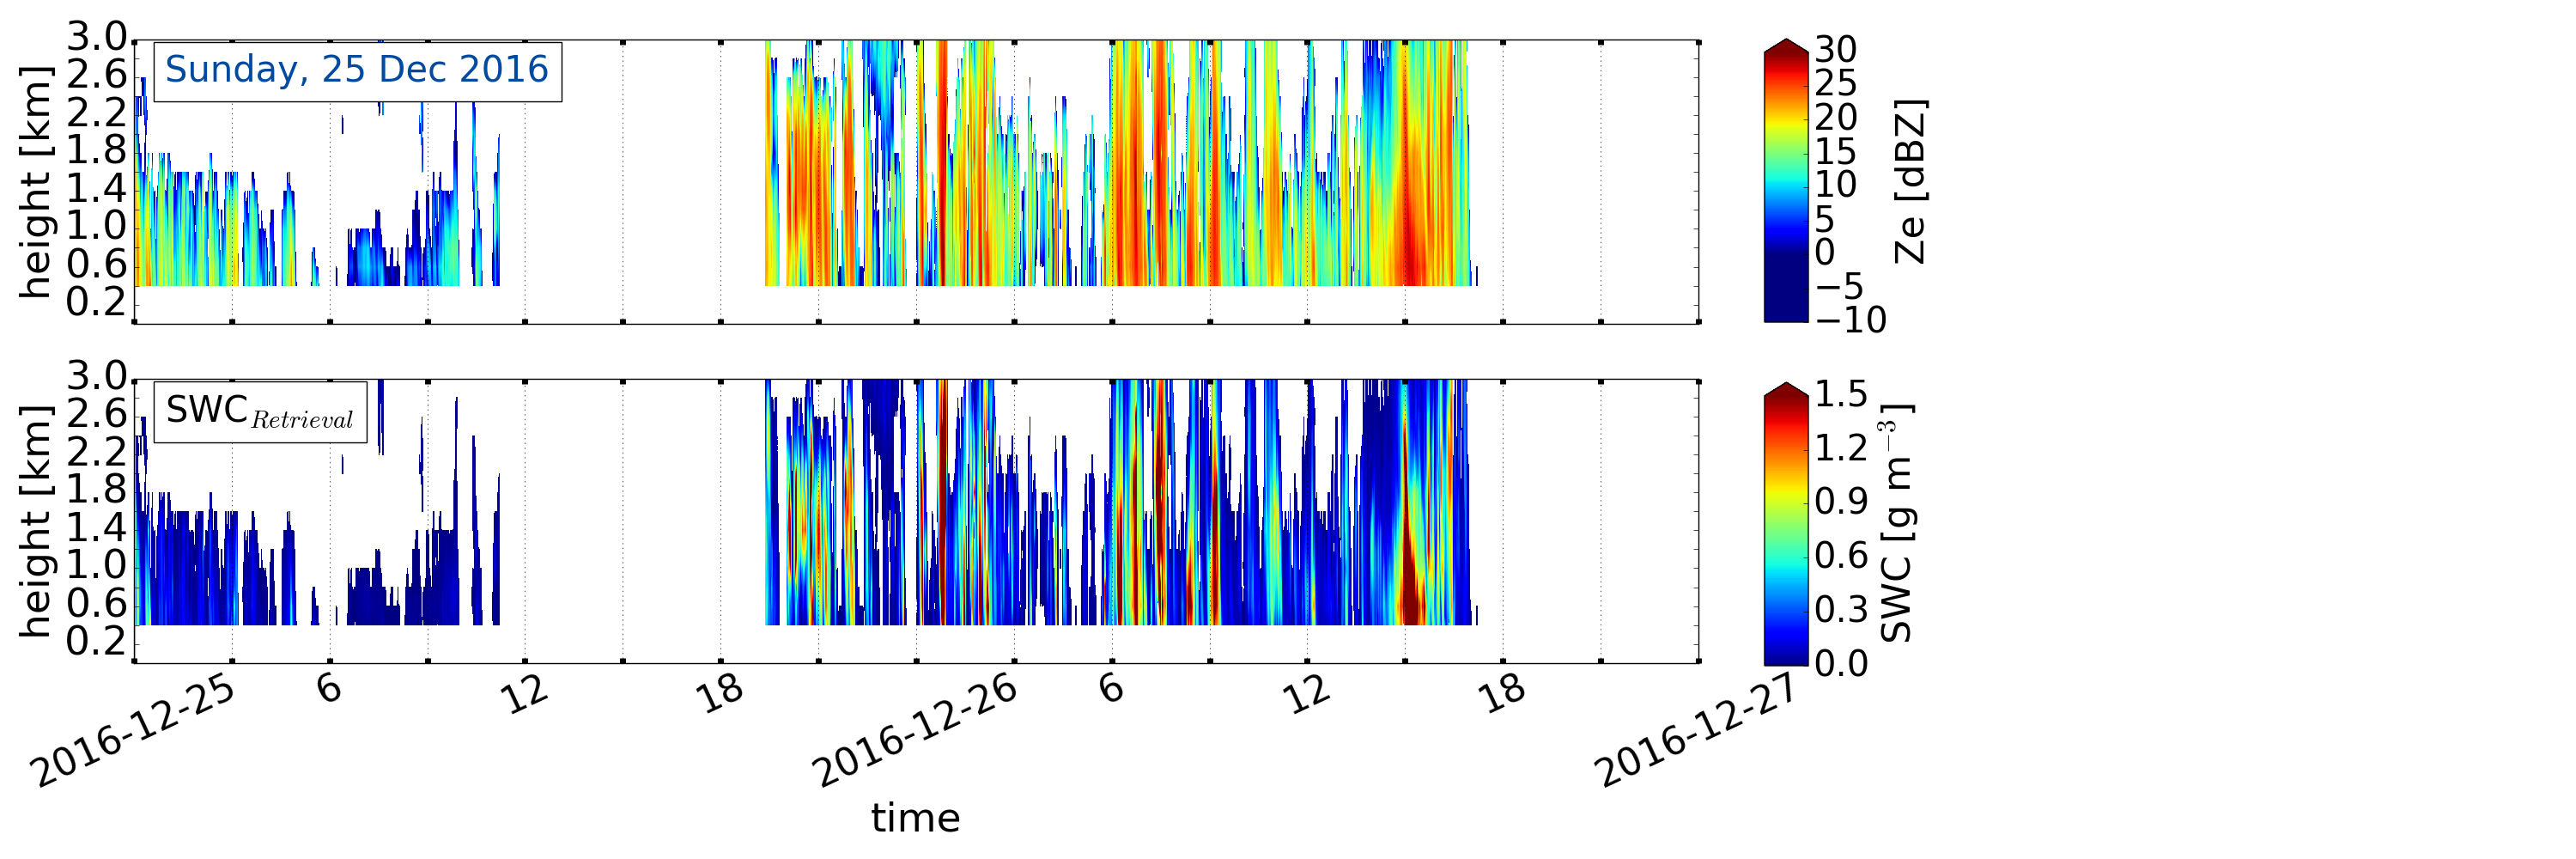
\includegraphics[trim={0.cm 2.2cm 19.cm 0.5cm},clip,width=0.9\textwidth]{./fig_obs_ret/20161225}
		\caption{}\label{fig:SWC:ret_25}
	\end{subfigure}
	% EM
	\begin{subfigure}[t]{\textwidth}
		\centering
		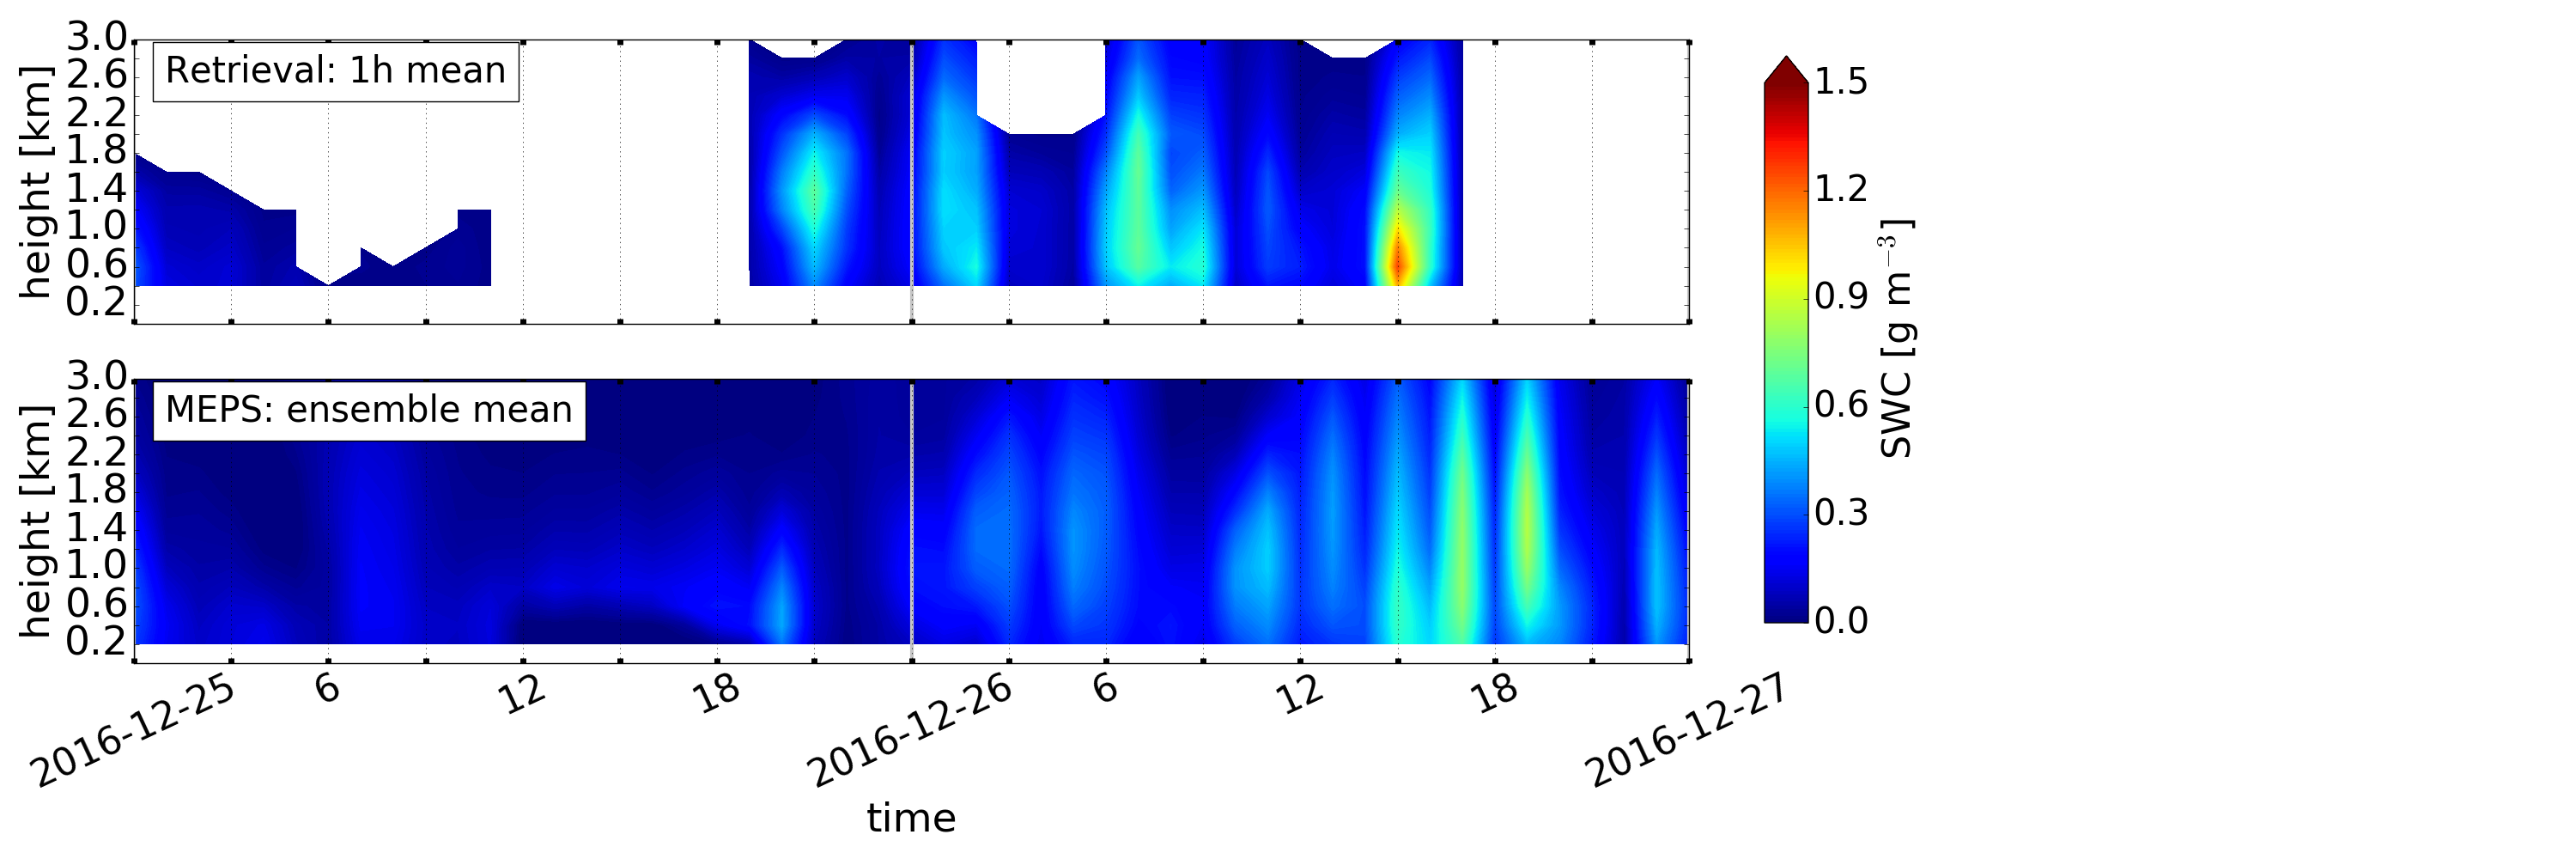
\includegraphics[trim={0.cm 2.2cm 19.cm 0.5cm},clip,width=0.9\textwidth]{./fig_vert_SWC_EM/20161225}
		\caption{}\label{fig:SWC_EM:25}
	\end{subfigure}
	% 3h
	\begin{subfigure}[t]{\textwidth}
		\centering
		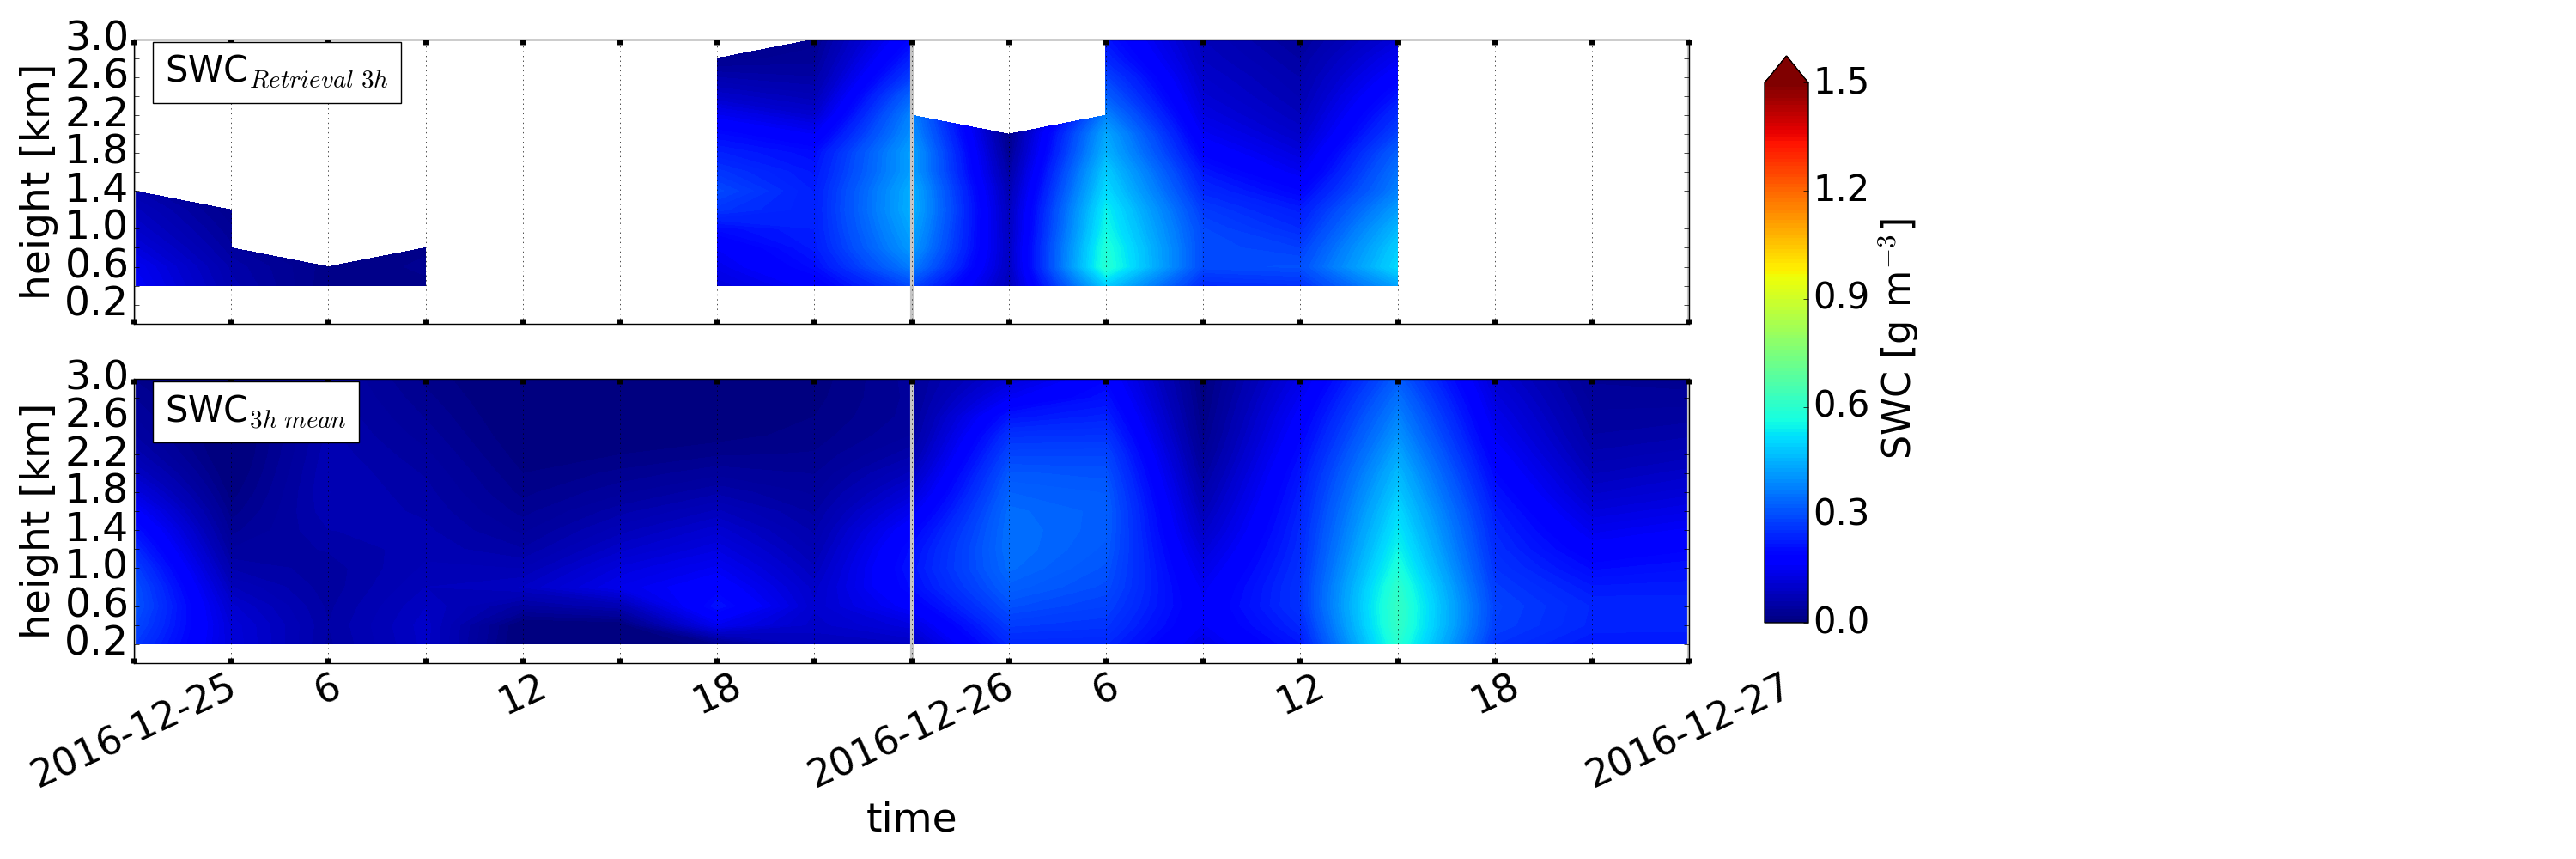
\includegraphics[trim={0.cm 0.8cm 19.cm 0.5cm},clip,width=0.9\textwidth]{./fig_vert_SWC_3h/20161225}
		\caption{}\label{fig:SWC3h:25}
	\end{subfigure}
	\caption{\textit{(Continued from previous page.)} Initialisation \SI{25}{\dec}.}
\end{figure}
%%%%%%%%%%%%%%%%%%%%%%%%%%%%%%%%%%%%%%%%%%%%%%%%%%%%%%%%%%%%%%%%%%%%%%%%%
\noindent
On \SI{23}{\dec} allow the surface observations to assume that the occluded front passed through between \SIrange{12}{21}{\UTC} (\Cref{fig:res:sfc_pres23}, \subref{fig:res:sfc_temp23}, \subref{fig:res:sfc_wd23}). The vertical observations at Haukeliseter show intense reflectivity and therefore more intense precipitation after \SI{16}{\UTC}. Another occlusion passed through on \SI{26}{\dec} shortly before \SI{15}{\UTC} which lasted until \SI{21}{\UTC}. The high reflectivity on both days shows the passage of the fronts and the associated precipitation. The wind on \SI{23}{\dec} was from the south, upslope (\Cref{fig:res:sfc_wd23}, \Cref{fig:site:kartverket}) which led to a more consistent storm structure. On \SI{25}{\dec} indicate \Cref{fig:res:sfc_wd25} and \subref{fig:res:sfc_ws25} strong wind observations from the west which led a consistent, but shorter storm structure in \Cref{fig:ret:refl25}. The orographic influenced wind and therefore a relation to the precipitation will be further assessed in \Cref{sec:res:oro_infl}. 
\\
\Cref{fig:SWC_EM:23} (lower panel) shows the one hourly averaged values over all ensemble members, neglecting not existing values. The forecast predicts the consistent storm pattern after \SI{16}{\UTC}, when initialised less than \SI{24}{\hour} before. Even the three hourly averaged forecast values show a response on the occurrence of the storm (\Cref{fig:SWC3h:23}, lower panel). That the \SI{3}{\hour} averages predicts the snow water content is related to the duration of the occlusion passage (between \SIrange{16}{23}{\UTC}).
%\\
%%%%%%%%% image SWC retrieval MEPS 26 %%%%%%%%%%%%%%
\begin{figure}\ContinuedFloat
	\centering
	% 25/12
	\begin{subfigure}[t]{\textwidth}
		\centering
		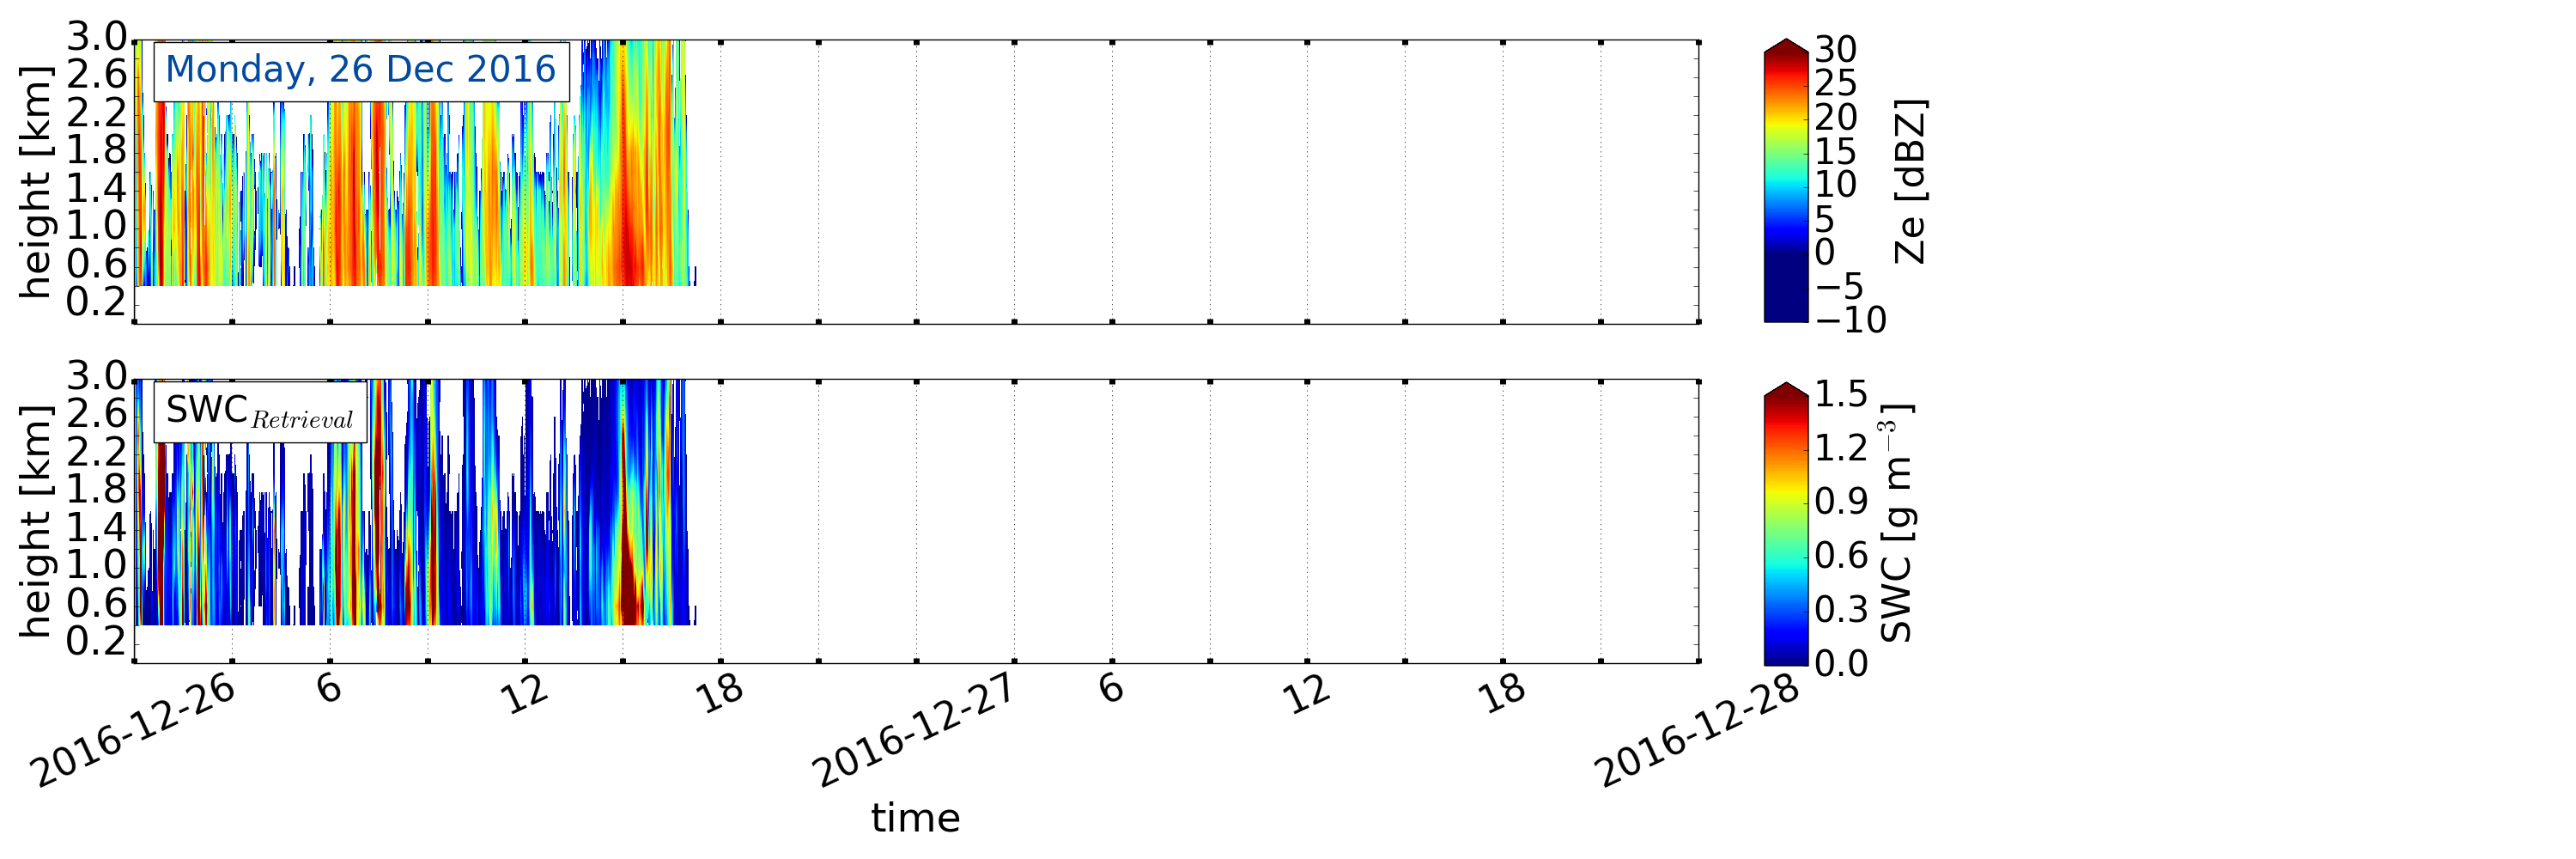
\includegraphics[trim={0.cm 2.2cm 19.cm 0.5cm},clip,width=0.9\textwidth]{./fig_obs_ret/20161226}
		\caption{}\label{fig:SWC:ret_26}
	\end{subfigure}
	% EM
	\begin{subfigure}[t]{\textwidth}
		\centering
		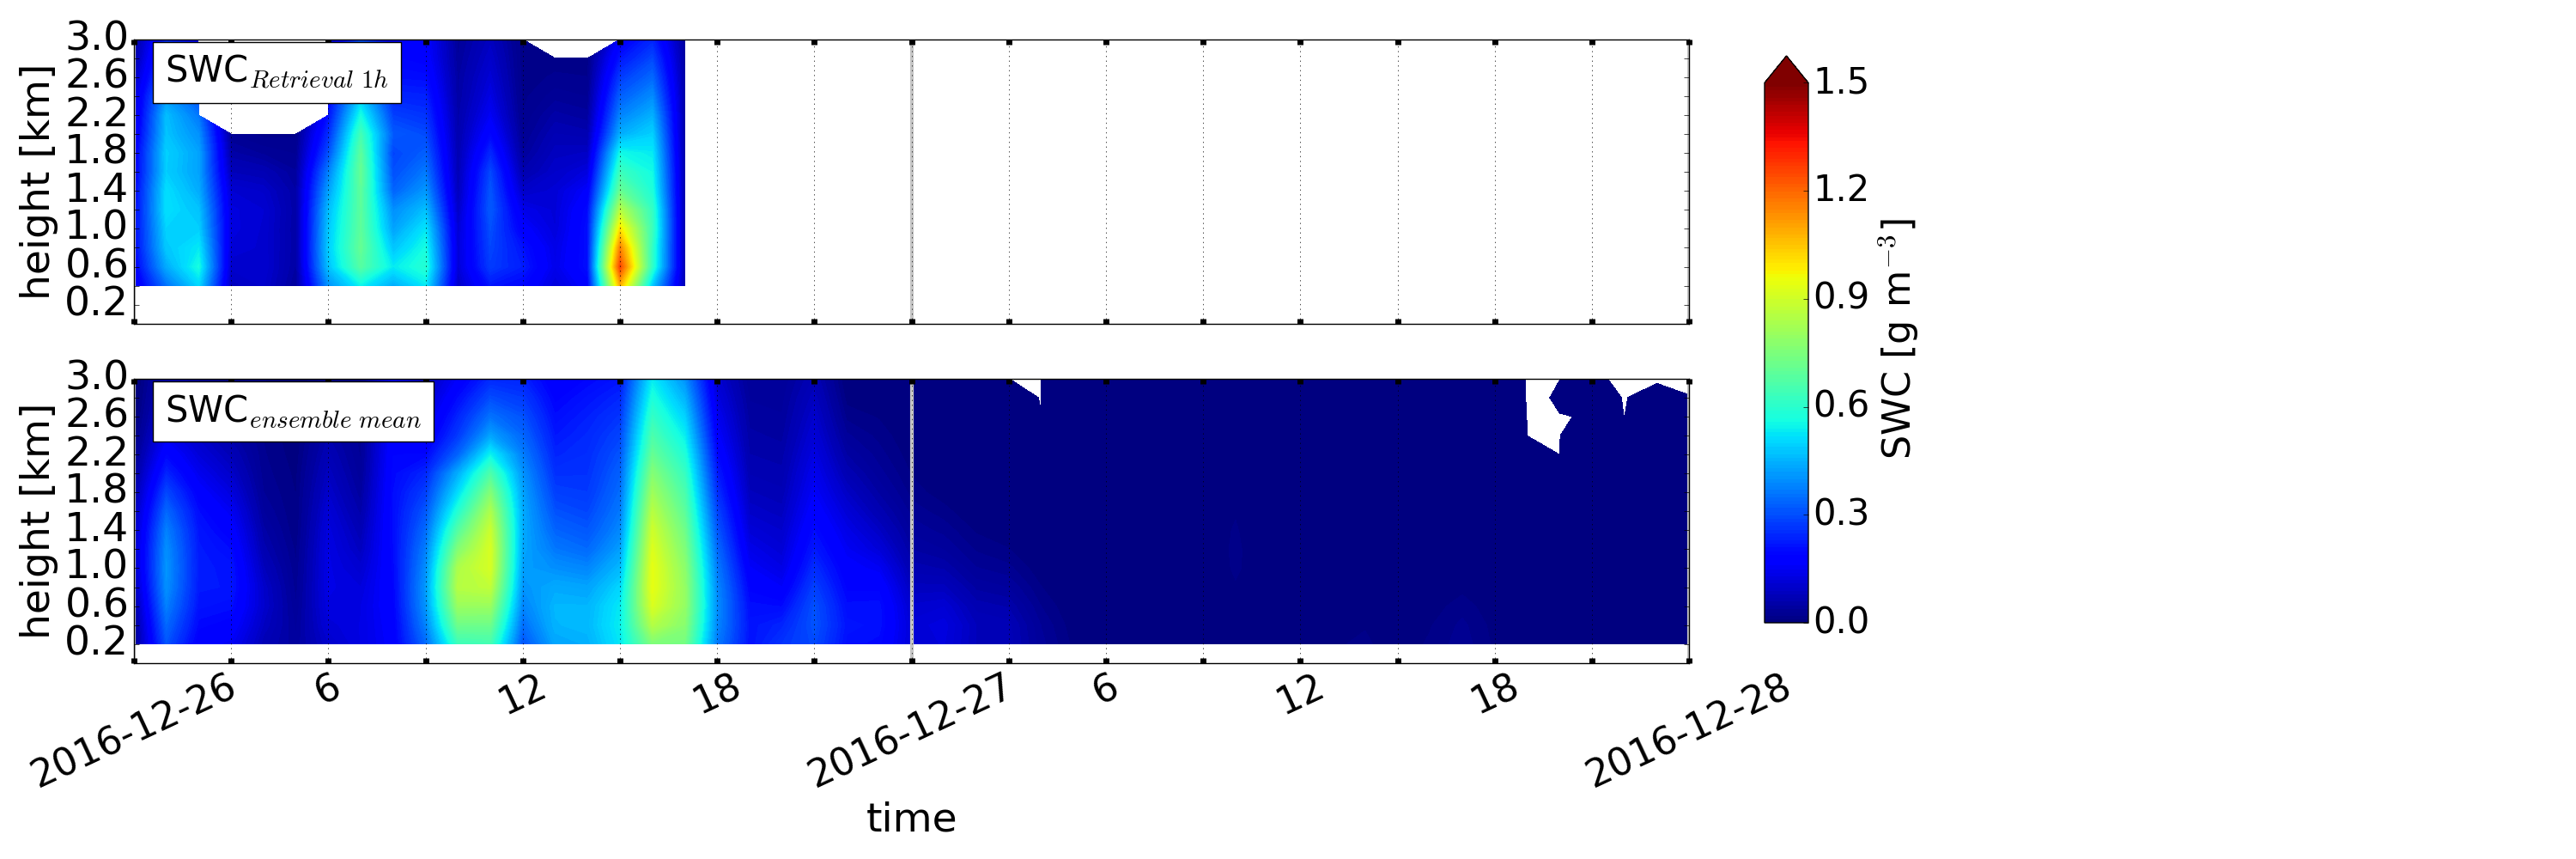
\includegraphics[trim={0.cm 2.2cm 19.cm 0.5cm},clip,width=0.9\textwidth]{./fig_vert_SWC_EM/20161226}
		\caption{}\label{fig:SWC_EM:26}
	\end{subfigure}
	% 3h
	\begin{subfigure}[t]{\textwidth}
		\centering
		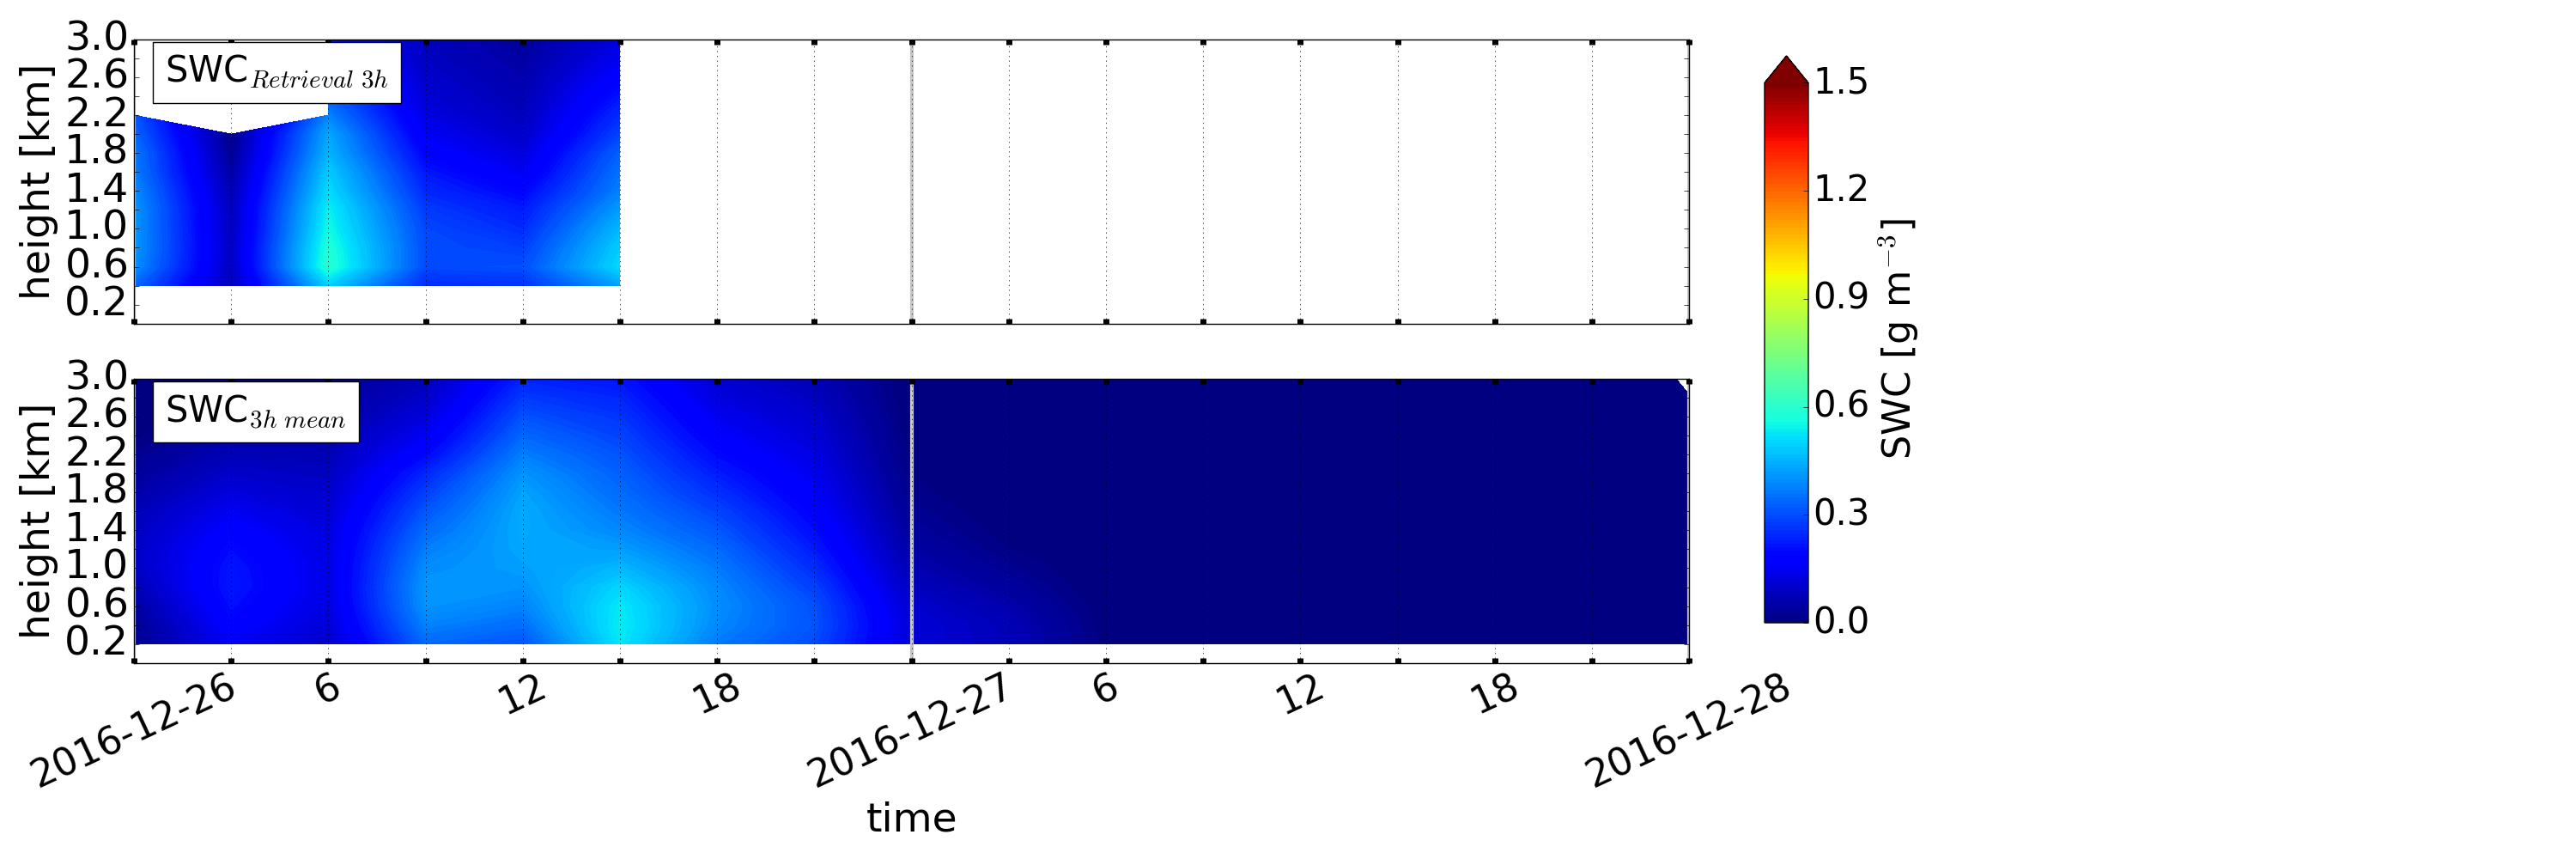
\includegraphics[trim={0.cm 0.8cm 19.cm 0.5cm},clip,width=0.9\textwidth]{./fig_vert_SWC_3h/20161226}
		\caption{}\label{fig:SWC3h:26}
	\end{subfigure}
	\caption{\textit{(Continued from previous page.)} Initialisation \SI{26}{\dec}.}
\end{figure}
%%%%%%%%%%%%%%%%%%%%%%%%%%%%%%%%%%%%%%%%%%%%%%%%%%%%%%%%%%%%%%%%%%%%%%%%%
In general, is the forecasted instantaneous snow water content amount weaker than the retrieved values on \SI{23}{\dec}. Hourly averages, only using the deterministic forecast and the first ensemble member show no occurrence of the occlusion passage on either day (\Cref{fig:SWC1h:23}, \subref{fig:SWC1h:25}, \subref{fig:SWC1h:26}). The variation of each ensemble member initialised on the respective day are given in \Cref{fig:EM09}. It shows that on \SI{23}{\dec} the first perturbed ensemble member does not exist and hence little snow water content is predicted for the ensemble means. A comparison with \SIlist{25;26}{\dec} shows the same result. Not much more snow water content is predicted when using the instantaneous values from the deterministic and first perturbed forecast (\Cref{fig:SWC1h:25}, \subref{fig:SWC1h:26}). 
\\ 
On \SI{26}{\dec} when the passage of the occlusion is predicted, the three-hourly instantaneous SWC (\Cref{fig:SWC3h:26}) as well as the average of all ensemble members (\Cref{fig:SWC_EM:26}) predict the frontal passage. 
Already initialisations \SI{39}{\hour} prior let assume that intense precipitation over a short time will occur. The variation of all members in \Cref{fig:EM09_25} and \subref{fig:EM09_26} indicate that almost all perturbed members would have predicted the precipitation around \SI{16}{\UTC}. The deterministic forecast shows in both cases the highest SWC vales when comparing to the perturbed members. But in \Cref{fig:SWC1h:25} and \subref{fig:SWC1h:26} is the amount of snow water content very weak. It shows better estimations for predicted snowfall amount when using either hourly or three hourly time resolution and all ten ensemble members to create the mean than forecasts for hourly averages with only the deterministic and first perturbed member.
Still the instantaneous average values of all ensemble members are much weaker than the retrieved SWC.
\\
Higher predicted values appear for deterministic forecasts than for any other ensemble member for initialisations on \SIlist{25;26}{\dec}. This bias might have led to an overestimation at the surface on \SI{26}{\dec}, where the deterministic forecast indicates higher values than the perturbed members (\Cref{fig:sfc_acc26}). 
\\
The \SI{25}{\dec} showed patterns of liquid precipitation (\Cref{fig:res:obs_masc}) with warm temperatures (\Cref{fig:res:sfc_temp25}) and high reflectivity (\Cref{fig:ret:refl25}) between \SIrange{12}{21}{\UTC}. To see if liquid precipitation was forecasted, the atmospheric cloud condensed water content and rainfall amount in model levels is summed. \Cref{fig:LWC:24} and \subref{fig:LWC:25} show liquid water content for initialisations at either \SI{24}{\dec} or \SI{25}{\dec}. 
Positive surface temperatures were forecasted between \SIrange{12}{21}{\UTC} (\Cref{fig:res:sfc_temp25}). Since MEPS forecasts the liquid layer correctly in depth and length it seems to be a good interaction between the surface model setting the vertical prediction. 
High reflectivity values in \Cref{fig:ret:refl25} are present around \SI{18}{\UTC} with layer thickness up to \SI{1.2}{\km}. \Cref{fig:LWC:24} or \subref{fig:LWC:25} show also a narrow thickness up to \SI{800}{\metre}. 
\\
%%%%%%% image liquid forecast 25 %%%%%%%%%%%%%%%%
\begin{figure}[t]
	\centering
	\begin{subfigure}[b]{\textwidth}
		\centering
		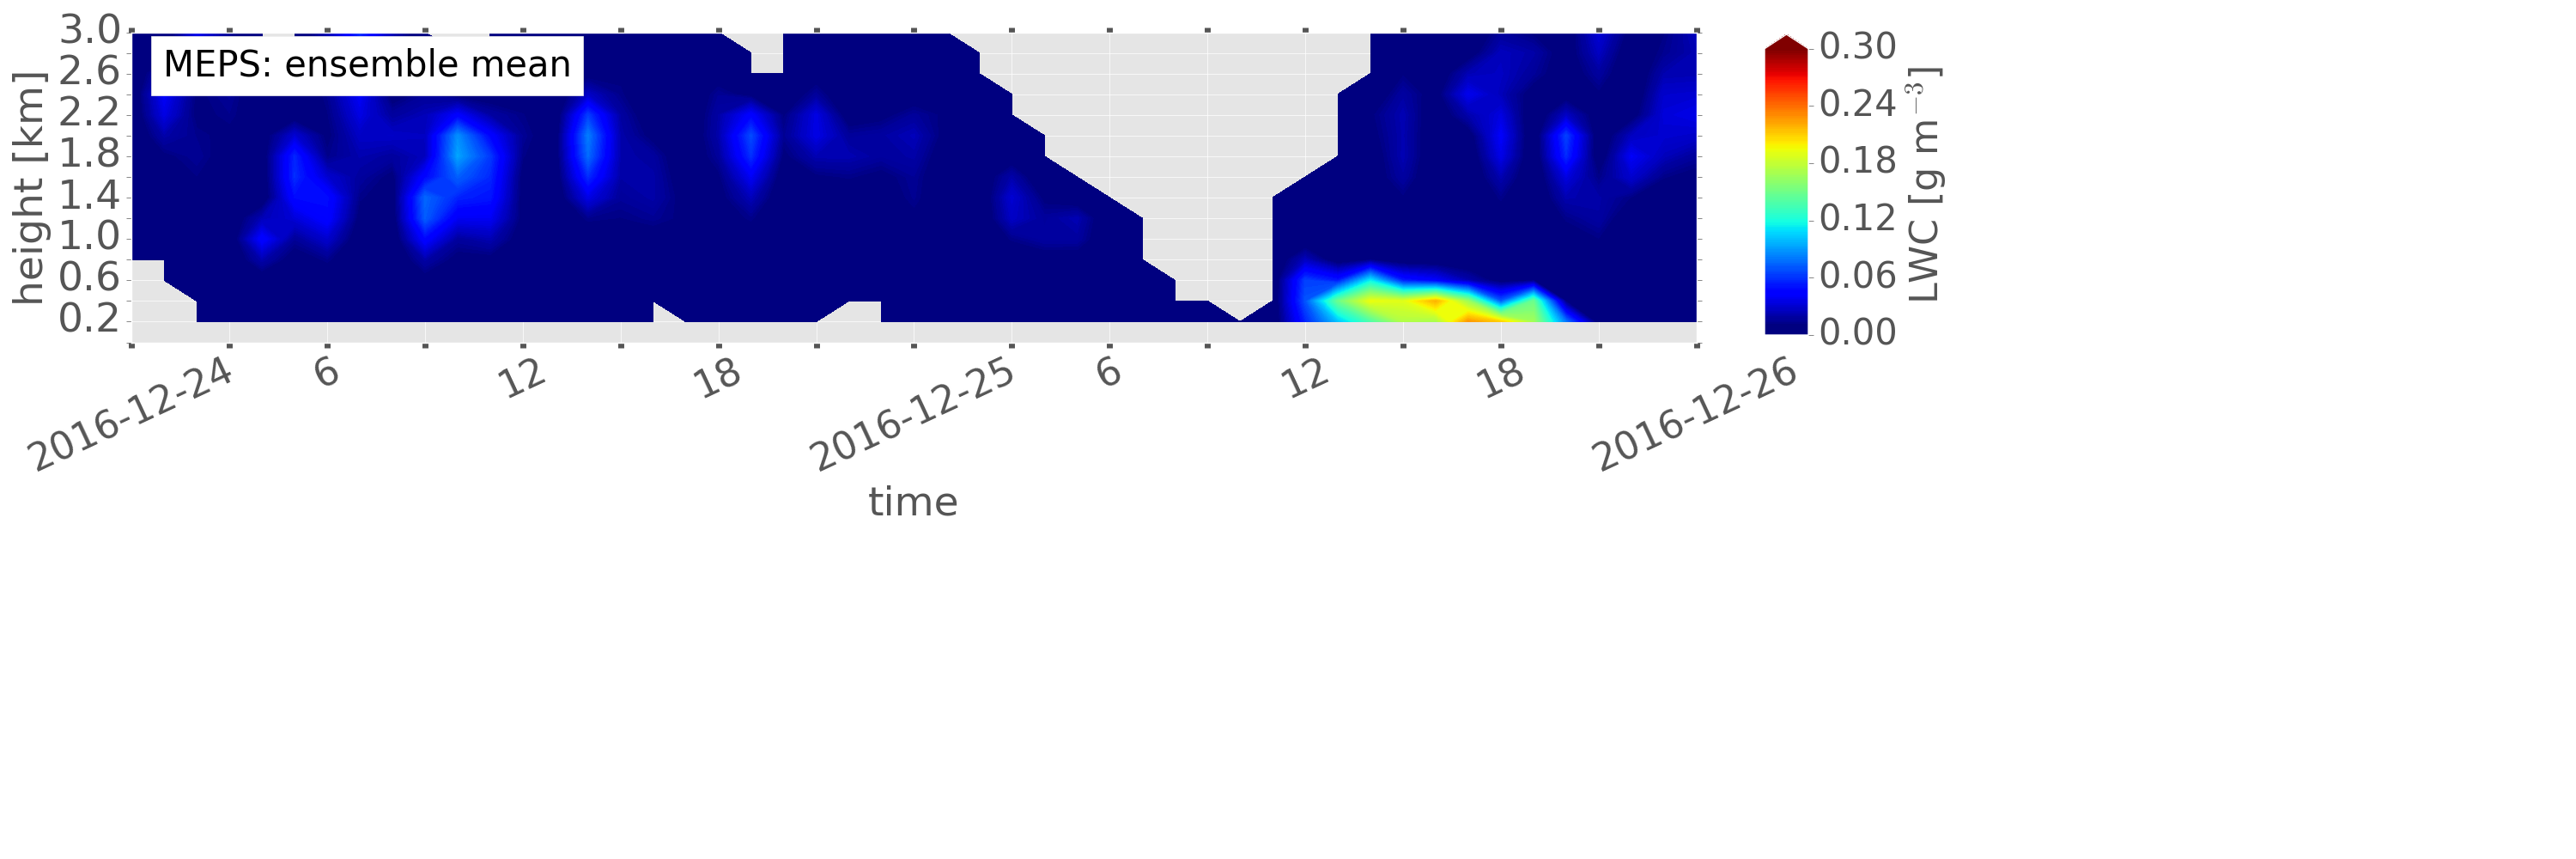
\includegraphics[trim={0.cm 1.9cm 26.5cm 0.4cm},clip,width=\textwidth]{./fig_vert_LWC_EM/20161224}
		\caption{}\label{fig:LWC:24}
	\end{subfigure}
	\begin{subfigure}[b]{\textwidth}
		\centering
		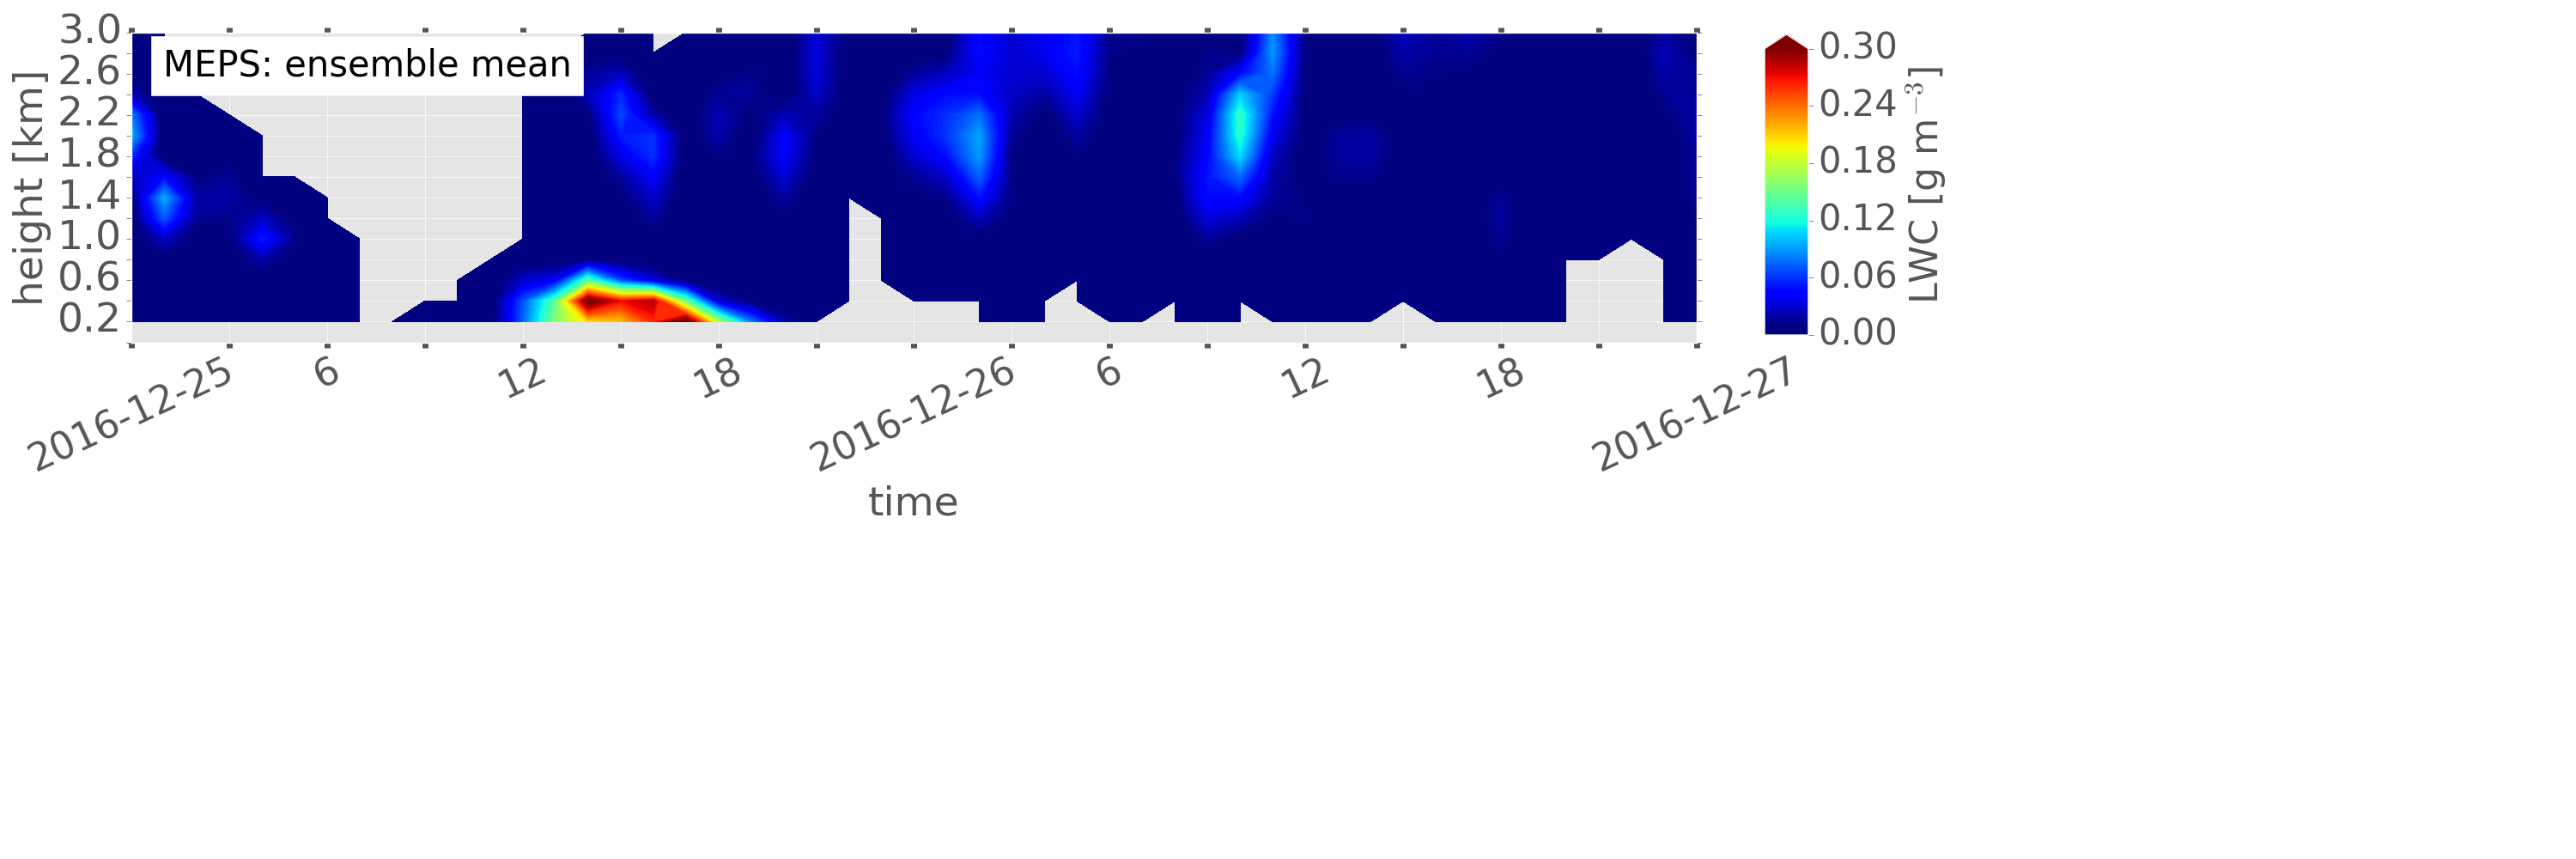
\includegraphics[trim={0.cm 1.9cm 26.5cm 0.4cm},clip,width=\textwidth]{./fig_vert_LWC_EM/20161225}
		\caption{}\label{fig:LWC:25}
	\end{subfigure}
	\caption{Upper panel: 200m hourly averaged LWC forecast from MEPS with all ensemble members, neglecting missing values.
		Lower panel: LWP from MEPS, initialised at \SI{0}{\UTC}. Black line represents the deterministic
		forecast, the doted blue line the ensemble mean and the grey lines the nine perturbed
		members.}\label{fig:LWC:2425}
\end{figure}
%%%%%%%%%%%%%%%%%%%%%%%%%%%%%%%%%%%%%%%%%%%%%%
A validation of how well the forecast performed is difficult to do at this state, since the time resolution of MEPS is coarse compared to the observations. For the first glance operates the forecast well when compared to vertical observations. One possibility to assess the variability of all ensemble member. 
\Cref{fig:ens_vari24,fig:ens_vari25,fig:ens_vari26} show the coefficient of variation for SWC, which is the standard deviation of the ten ensemble members divided by the mean of all ensemble members. This coefficient gives the possibility to compare the SWC results for different days with different values. It also shows if the ensemble spread (standard deviation of all ensemble members) is low the SWC is does not need to be less variable.
%\\
\noindent
One question to answer in this work is if the operational model MEPS gets large scale features correctly. As discussed here and in \Cref{sec:res:large_scale_sfc} it seems that the model is able to cover the development of large scale features and its associated precipitation. Even with the intensification of the storm seems MEPS to be able to predict extreme events such as the Christmas event. 
MEPS is also able to distinguish between liquid and solid precipitation in layer thickness and duration. This can be major approach since a change in temperature and associated precipitation transformation can lead to major risks in the Norwegian mountains, especially during winter. With the knowledge more than \SI{24}{\hour} prior risk notice can be send out to the population and rescue teams can prepare better. Furthermore, roads and train tracks can be closed to increase the safety of people.
\\
\textcolor{red}{I'm not sure if the above mentioned should be here?! }

%%%%%%%%%%%%%%%%%%%%%%%%%%%%%%%%%%%%%%%%%%%%%%%%%%%%%%%%%%%%%%%%%%%%%%%%%%
%%%%%%%%% Local affects %%%%%%%%%%%%%%
\section{Orographic influence on precipitation}\label{sec:res:oro_infl}
It has shown, that wind plays an important role at the Haukeliseter measurement site, since it is suspended to high wind speeds during the winter. The mountain plateau is surrounded by higher mountains to the west and more open to the south east \citep{wolff_measurements_2013,wolff_derivation_2015}). The correlation between wind speed observations and forecast have shown an overestimation throughout the event (\Cref{fig:scat:ws2123} and \subref{fig:scat:ws2426}). It seems, that wind direction plays an important role too, at the Haukeliseter site. 
\\
During \SIrange{24}{26}{\dec} was the wind constantly from the west with higher wind speeds observed than during \SIrange{21}{23}{\dec} (\Cref{fig:res:sfc_wd23}, \subref{fig:res:sfc_wd25}, \subref{fig:res:sfc_wd26}; \Cref{fig:res:sfc_wd21}, \subref{fig:res:sfc_wd22}, \subref{fig:res:sfc_wd24}; \Cref{fig:res:sfc_ws23}, \subref{fig:res:sfc_ws25}, \subref{fig:res:sfc_ws26}, and \Cref{fig:res:sfc_ws21}, \subref{fig:res:sfc_ws22}, \subref{fig:res:sfc_ws24}). \Cref{fig:scat:wd2123} and \subref{fig:scat:wd2426} indicate a better agreement between the forecasted and observed wind directions when precipiation overestimation occured. During \SIrange{24}{26}{\dec} were the observed wind speeds higher than on the previous days, and as \Cref{fig:scat:ws2123} and \subref{fig:scat:ws2426} present is the correlation between observation and forecasts lower during high wind speeds.
\\
While the wind direction of MEPS has a good agreement shows the wind speed larger values over all days. Although MEPS includes ten perturbed ensemble members the insufficiency of AROME-MetCoOp too high wind prediction in extreme situations is not resolved. The regional model wind prediction is still dependent on the intensity of the storm. As \cite{muller_arome-metcoop:_2017} also mentioned are higher wind speeds in general better forecasted in AROME-MetCoOp than in ECMWF. 
%%%%%%%%%%%%%%%%%%%%%%%%%%%%%%%%%%%%%%%%%%%%%%%%%%%%%%%%%%%%%%%%%%%%%%%%%%


